\subsection{Photometric classification}

\myparagraph{Method}

The aim of this investigation is to analyse the affect a particular cadence has
on one's ability to photometrically classify supernova. This investigation has been carried out by the
developers of {\tt snmachine}, a DESC product that is used as a photometric
classification pipeline \cite{lochner2016photometric}.

The motivation for this work comes from the desire to identify as many \sne in
order to help constrain the nature of Dark Energy.
LSST will observe many more Supernova than ever before, but at a rate that is
not feasible for all of these transients to be spectroscopically followed up and
classified. Thus, the ability to classify these objects photometrically will be very
important. If one can obtain a greater set of \sne, an updated Hubble
digram plot can be produced and the fundamental parameters of the cosmological
model can be tested further.

In order to conduct this analysis, use of
{\tt SNANA}\cite{kessler2009snana}, has been employed to generate the latest light curves that
correspond to different cadences runs from \opsim outputs. The generated light
curves are then used as inputs in the {\tt snmachine} pipeline.

By interpolating the sampled light curved with Gaussian processes and then
applying a wavelet decomposition to these interpolated light curves, one obtains features
that could be provided to a classifier, in this case a Random Forest algorithm.
For performance, the dimensions of these features were reduced further with a principle
component analysis and then these reduced features were provided as inputs to the algorithm.
To ensure a controlled test,
for each cadence run, a classifier was trained on 2000 light
curves only and then tested on the remaining set of light curves that were in the
corresponding dataset produced from {\tt SNANA}, in relation to specific
\opsim cadence simulation. The results for which are shown in
Figure~\ref{fig:rocs}.
The performance of the interpolation is directly affected by the amount of
samples one has on the light curve. More samples improve the reliability of the
Gaussian processes and thus provide better features via the wave
decomposition.

Therefore, it can be understood that in order to classify transients, short
sampling of a light curve is important. This is particularly crucial for early classification
leading to possible spectroscopic follow up.

\myparagraph{Results}

\begin{figure}
  \centering
  \subfigure[DDFY1]{\label{fig:ddfy1}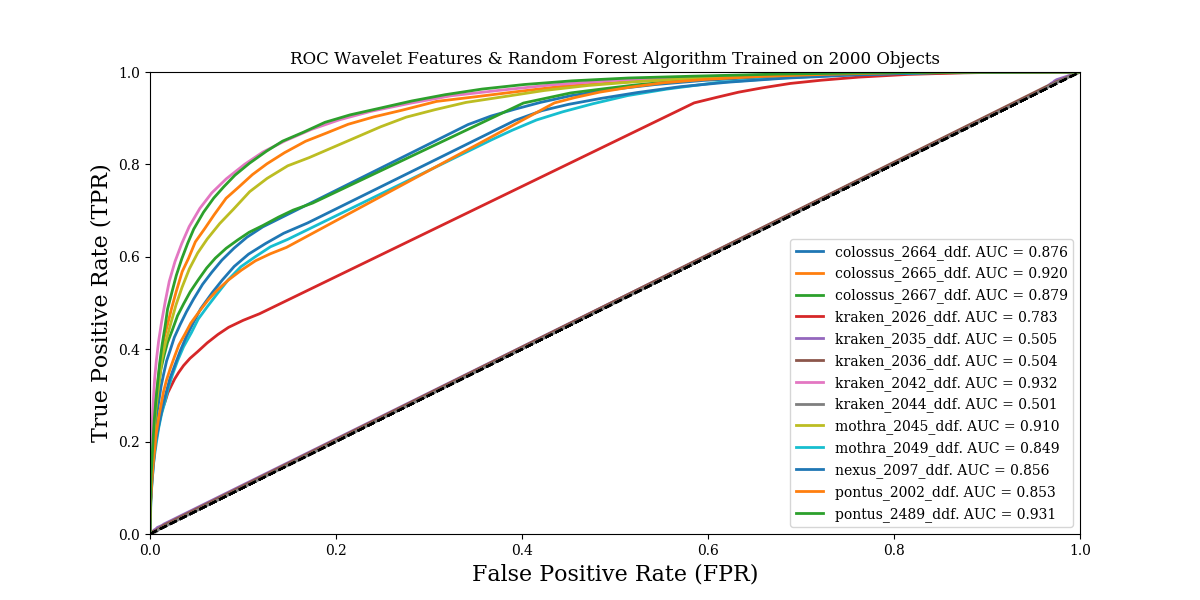
\includegraphics[width=0.8\textwidth]{classification/photometric_classification_roc_results_ddfY1.png}}
  \subfigure[DDFY10]{\label{fig:ddfy10}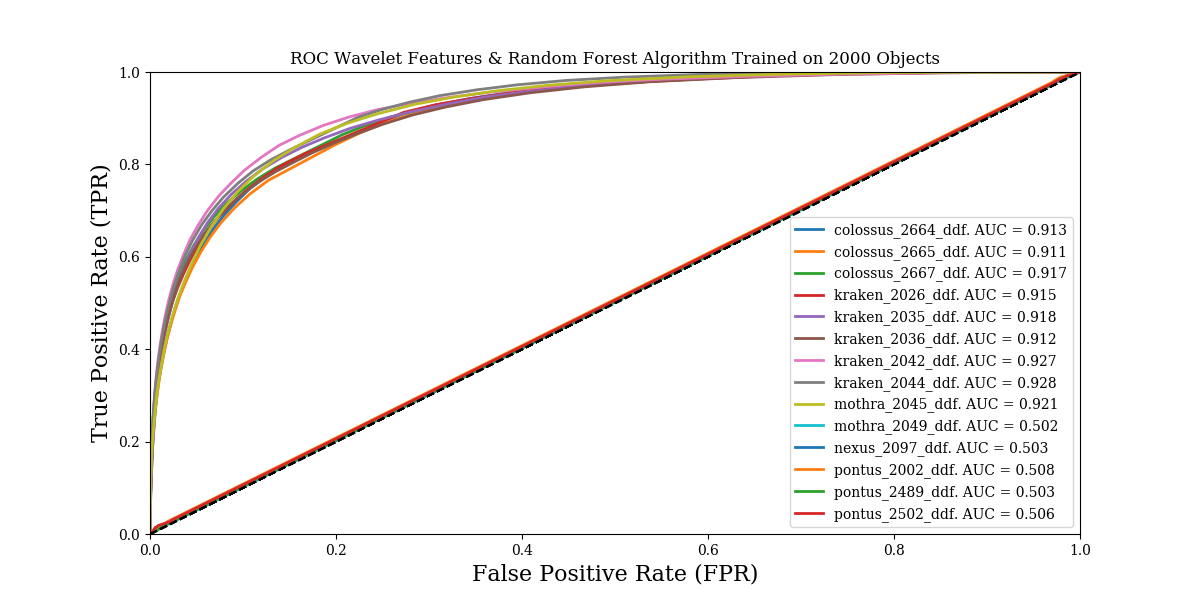
\includegraphics[width=0.8\textwidth]{classification/photometric_classification_roc_results_ddfY10.png}}
  \caption{Comparison for the DDFY1 and DDFY10 ROC curves}\label{fig:rocs}
\end{figure}

Figure \ref{fig:ddfy1}~shows the comparative classification performance between 13 cadences for the Deep
Drilling Fields of Year 1 whereas Figure \ref{fig:ddfy10}~compares the same
cadences for the Deep Drilling Fields over the entire survey.

The area under the Receiver Operating Characteristic (auROC) curves were chosen as the metric
to evaluate the performance. It was felt this single scalar would be most useful
for being able to differentiate the ability of the various cadence strategies
to perform photometric classification.

\myparagraph{Conclusion}

The results for the DDFY1 case show a significant difference in classification
performance between cadences, with {\tt kraken\_2042} being most favourable.
This cadence has single 30 second snapshots in all bands, thus providing better
sampling along the light curve in all bands. This is one of the elements that could explain
the good performance, and further studies are being carried out to explore which
other elements of cadence result in better classification performance.

If we look at the 10 year survey results, it can be seen there is
little that differentiates the cadences in regard to classification performance.
However, the best performing cadence models are {\tt kraken\_2044} and
{\tt kraken\_2042} which again can be expected from the discussion above.

Further analysis was also done on Wide-Fast-Deep (WFD) cadence runs with work in
progress for models trained on DDF and then tested on WFD.

This research can be taken further in several ways and there are plans to
continue this analysis for new \opsim simulation runs.  In addition, it is
of interest to investigate how the classification performance changes through
time and to compare the results for earch year of the survey. Furthermore,
varying the training set size could have an impact on how well one does for
classification and so this is an area for possible further study.
Finally it would be beneficial to understand how the individual properties of each cadence
strategy affect classification.
